\section{Iteration \#1 -- Pseudo-Pyramid Tree}
\label{sec:iteration1}

This iteration deals with the low-level implementation details of the Pseudo-Pyramid Tree index structure. Different optimisation techniques are applied to the structure and multiple implementations of the Pseudo-Pyramid Tree are analysed to determine which is the fastest.

\subsection{Initial Pseudo-Pyramid Tree Implementations}

The Pseudo-Pyramid tree's reduction from $d$ dimensions to one can be seen as a hashing function, where the one-dimensional value acts as the hash to use when searching a hash table. The Initial implementation of the structure stores all the points in a single array, which hashes each point to an integer representation that acts as the key to a bucket stored in a hash map (specifically \texttt{boost::unordered\_map}, part of the Boost\footnote{\url{http://www.boost.org/}} library). A bucket is an array that contains indices to points in the single point array. Another array is used to store the sums of all stored points. This is used to speed up point queries, by comparing the sums (one comparison) of the input point to the points in a bucket. A full point comparison ($d$ comparisons) only needs to be performed if the sums match up.

No \texttt{delete} operation was provided in the original implementation of the Pseudo-Pyramid Tree, so a \texttt{delete} procedure had to be added. To delete a point $p$, the point is first hashed and the bucket containing the point is found. The index pointing to $p$ in the bucket is removed from the bucket, but the actual point itself is not removed from the point array. In other words, the memory is never released until the whole structure is deleted. This makes the structure useful for batch computation because it can be discarded straight after a task, releasing all allocated memory then. However, if the structure is used as part of a long-running process then this is not suitable because there is the potential to run out of memory.  One of the core assumptions of this project is that data may be dynamic, meaning points may be inserted and deleted frequently. For this reason, another implementation of \texttt{delete} which releases memory has been developed.

The \textbf{Rebuild Index Pseudo-Pyramid Tree} uses a different strategy for releasing memory for unused points. Instead of defragmenting the array by performing a sequence of array deletions when $R + 1$ elements are marked for deletion, the entire structure is rebuilt. This new cleanup procedure starts by clearing the structure and incrementally building the new structure by only adding points \textit{not} marked for deletion. $n - R$ points will be re-inserted and insertion in the worst case is $O(n)$, meaning the worst case complexity of \texttt{delete} is $O((n - R)n)$. The larger $R$ is, the less time it takes to perform this procedure but a larger amount of allocated memory goes unused at a time.

\subsection{Accelerating Hash Function}

The existing Pseudo-Pyramid tree hash function is an $O(d^2)$ operation because of the inner loop that computes $\prod_{j=0}^{i}{\lbrack m_j \rbrack}$. If $m$ is changed during the structure's lifetime, the structure must be rebuilt. Otherwise the one-dimensional value of a point could change and stored points can become inaccessible. Therefore, $m$ is constant in the Pseudo-Pyramid Tree. This allows the hash function to be executed in $O(d)$ time by \textit{pre-computing} $\prod_{j=0}^{i}{\lbrack m_j \rbrack}$. This pre-computation happens when the Pseudo-Pyramid Tree is initialised. The new hash function is given in Equation \ref{eq:new-pseudo-pyramid-hash}.

\begin{multline}\\
	h(p) = \sum_{i = 0}^{d} { \lbrack \texttt{toInt}( h_i(p) \times m_i ) \times M_i \rbrack } \\
	\text{where } M_i = \prod_{j=0}^{i}{\lbrack m_j \rbrack} \;\;\; \text{for} \; 0 \leq i \leq d \\
	\label{eq:new-pseudo-pyramid-hash}
\end{multline}

Table \ref{tab:new-pseudo-pyramid-hash} shows operation execution time of the Batch Pyramid Tree using the original $O(d^2)$ hashing function and the new $O(d)$ function on a 200D dataset. Figure \ref{fig:new-pseudo-pyramid-hash} plots the performance of the Pseudo-Pyramid Tree with both hash functions alongside Sequential Scan, showing execution time against dimensionality. From the plot, it is clear that the new hashing function is superior. The old hash function caused the Pseudo-Pyramid Tree to be slower than Sequential Scan when the dimensionality exceeded a certain number ($\approx 57$). The new hash function makes the structure significantly faster than Sequential Scan, even for dimensions as high as 200.

\begin{table}
	\centering
	\begin{tabular}{|l|l|l|}
		\hline
		\textbf{Operation} & \textbf{$O(d^2)$ Function} & \textbf{$O(d)$ Function} \\
		\hline
		Delete & 0.730777 & 0.027272  \\
		Insert & 1.46412 & 0.012032 \\
		Point Query & 0.731469 & 0.007477 \\
		\hline
	\end{tabular}
	\caption{Total Execution Time (in seconds) of Rebuild Pseudo-Pyramid Tree Using $O(d^2)$ and $O(d)$ Hash Function (200D Randomly Uniform Dataset, 10,000 operations each)}
	\label{tab:new-pseudo-pyramid-hash}
\end{table}

\begin{figure}
	\centering
	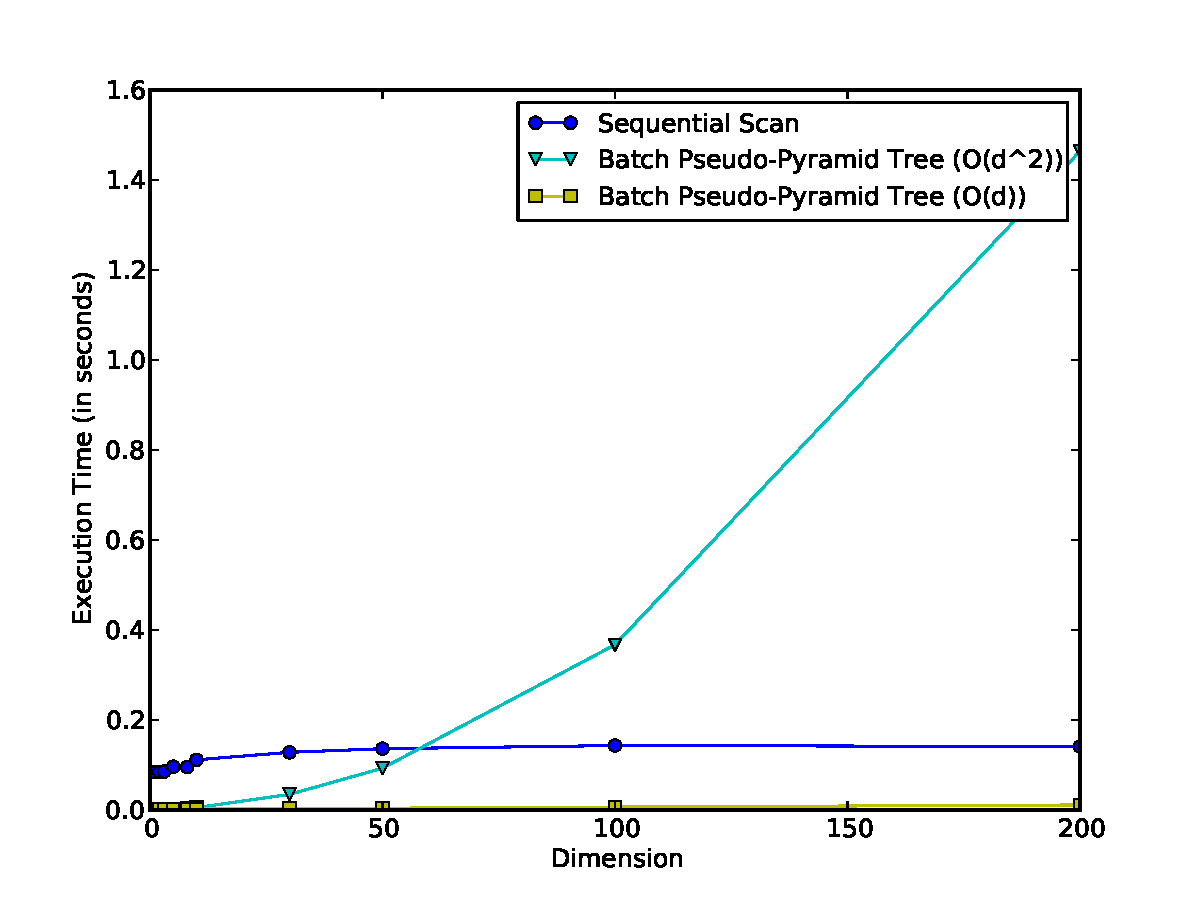
\includegraphics[scale=0.5]{figures/performance_analysis/iteration_1/new_pseudo-pyramid_hash_performance.pdf}
	\caption{\texttt{insert} Performance on Random Uniformly Distributed Datasets of Varying Dimensions}
	\label{fig:new-pseudo-pyramid-hash}
\end{figure}

\subsection{SSE Optimisation}

Since optimising the hashing function resulted in a massive speed increase, it was decided that the function would be parallelised using SSE. Considering point equality is used throughout all the index structures and will be executed many times if there are large buckets in the Pseudo-Pyramid Tree, it is worth optimising to see if there is any major speed-up. Point equality, like the hashing function, is an $O(d)$ operation. In both operations, there is loop which iterates once for each dimension, where each iteration is independent of the others. If 32-bit floating point numbers are used, then four dimensions can be processed at once using 128 bit SSE registers. Since each operation does not spend their entire time hashing or comparing points, it is not expected that a speedup of four can be achieved.

Table \ref{tab:pseudo-pyramid-sse} shows the execution times of the Pseudo-Pyramid Tree with and without SSE optimisation for the hash function and point equality. Across all three operations, the speedup averages to approximately $1.97$ when there are 200 dimensions. Note that if the number of dimensions is less than four, there is little benefit using the 128-bit SSE registers, so the structure uses the sequential hashing function and point equality check.

\begin{table}
	\centering
	\begin{tabular}{|l|l|l|}
		\hline
		\textbf{Operation} & \textbf{Without SSE} & \textbf{With SSE} \\
		\hline
		Insert & 0.092386 & 0.027601 \\
		Delete & 0.035891 & 0.012370 \\
		Point Query & 0.026402 & 0.007745 \\
		\hline
	\end{tabular}
	\caption{Total Execution Time (in seconds) of Rebuild Index Pseudo-Pyramid Tree With and Without SSE Optimisation (200D Randomly Uniform Dataset, 10,000 operations each)}
	\label{tab:pseudo-pyramid-sse}
\end{table}

\subsection{Bucket Pseudo-Pyramid Tree}

The index-based variants require the CPU to fetch two elements from main memory for each point in a bucket -- the index of a point and the point itself. This also results in more random accesses in the single point array, potentially causing more cache misses, because a bucket's indices may point to distant parts of the large point array. Furthermore, having a large point array makes \texttt{delete} operations difficult to perform cheaply.

The Bucket Pseudo-Pyramid Tree implementation does not use a single array to store the points. Instead of buckets containing an array of point indices, it has an array of actual points. The goal of this variant is to increase \textbf{cache coherency} when searching a bucket, since the point array can be searched sequentially and only one memory read is required. No cleanup procedure is necessary because the memory for a point is released immediately after it's removed, by simply erasing it from the corresponding bucket's array (which is much smaller than an array containing \textit{all} the points). However, \texttt{delete} is still an $O(n)$ operation since the worst case is when a single bucket stores all $n$ points.

The order the points are stored in a bucket do not matter, the C++ \textit{erase-remove} idiom has been used to delete elements from the bucket arrays. This idiom swaps the element to delete with the last element in the array, removing the desired element when it's at the end of the array. This means there is no need to move any elements in the array to fill the gap created by removing an element, since the element removed is always at the end of the array.

\subsection{Splay Pseudo-Pyramid Tree}

Another implementation of the Pseudo-Pyramid Tree, which does not use a hash map as the underlying one-dimensional index structure, was developed. Instead, the implementation uses a a splay tree. The splay tree is a self-adjusting variant of the binary search tree that uses a \textit{splaying} operation (a heuristic) to allow faster access to recently accessed elements. \cite{splay-tree}. The splaying operation achieves this by performing a series of tree rotations that move a given node up to the root of the tree. Through amortised analysis and empirical experiments, it has been shown splay trees can be more efficient than standard binary trees for a series of non-random operations \cite{splay-tree}, despite the asymptotic worst case bound being worse than binary search trees.

This implementation shall be called the \textbf{Splay Pseudo-Pyramid Tree}. Nodes in the Splay Pseudo-Pyramid Tree correspond to individual buckets in the Bucket Pseudo-Pyramid Tree, meaning each node can store multiple points. Since the splay tree is implemented as a collection of heap-allocated nodes with pointers to link them, deletions are cheap as a low amount of memory needs to be de-allocated per \texttt{delete} operation. The aim is that this, combined with the self-adjusting nature of the splay tree, will produce a Pseudo-Pyramid Tree implementation that is more efficient for non-random operations used in real applications.

\subsection{Performance Timings}

All implementations of the Pseudo-Pyramid Tree hash $d$-dimensional points to a one-dimensional value, which is used as a key to search for a given point in a one-dimensional structure. What varies is how points are deleted and which underlying one-dimensional structure is used.

The remaining Pseudo-Pyramid implementations and the two baselines, Sequential Scan and Octree, were timed with the full collection of synthetic and real datasets. The parameter $B$, which controls how the Pseudo-Pyramid Tree hashes points, was set to 300,000. This value was found to produce the fastest speed on the target hardware through trial and error. $R=3000$ was used for the Rebuild Index Pseudo-Pyramid Tree, which caps the amount of unused memory the structure allocates at 3000 points. When 3001 points are removed, the rebuild procedure will be executed.

Plots with point dimensionality against execution time for \texttt{insert} and \texttt{delete} are shown in Figure \ref{fig:perf1-dimensionality}. Plotting point query execution time adds little information, because both of these operations will perform a point query anyway (due to Core Assumption (4)). The total execution times of all three operations of each structure, for synthetic data (uniform, skewed and clustered distributions) where the dimensionality is varied, is shown in Tables \ref{tab:perf1-dimensionality-uniform}, \ref{tab:perf1-dimensionality-skewed} and \ref{tab:perf1-dimensionality-clustered} in Appendix \ref{chap:performance-timings}. For brevity, they are not included in the main report.

\begin{figure}
	\makebox[\textwidth][c]{%
		\begin{subfloat}[\texttt{insert}\label{fig:perf1-dimensionality-insert}]{%
			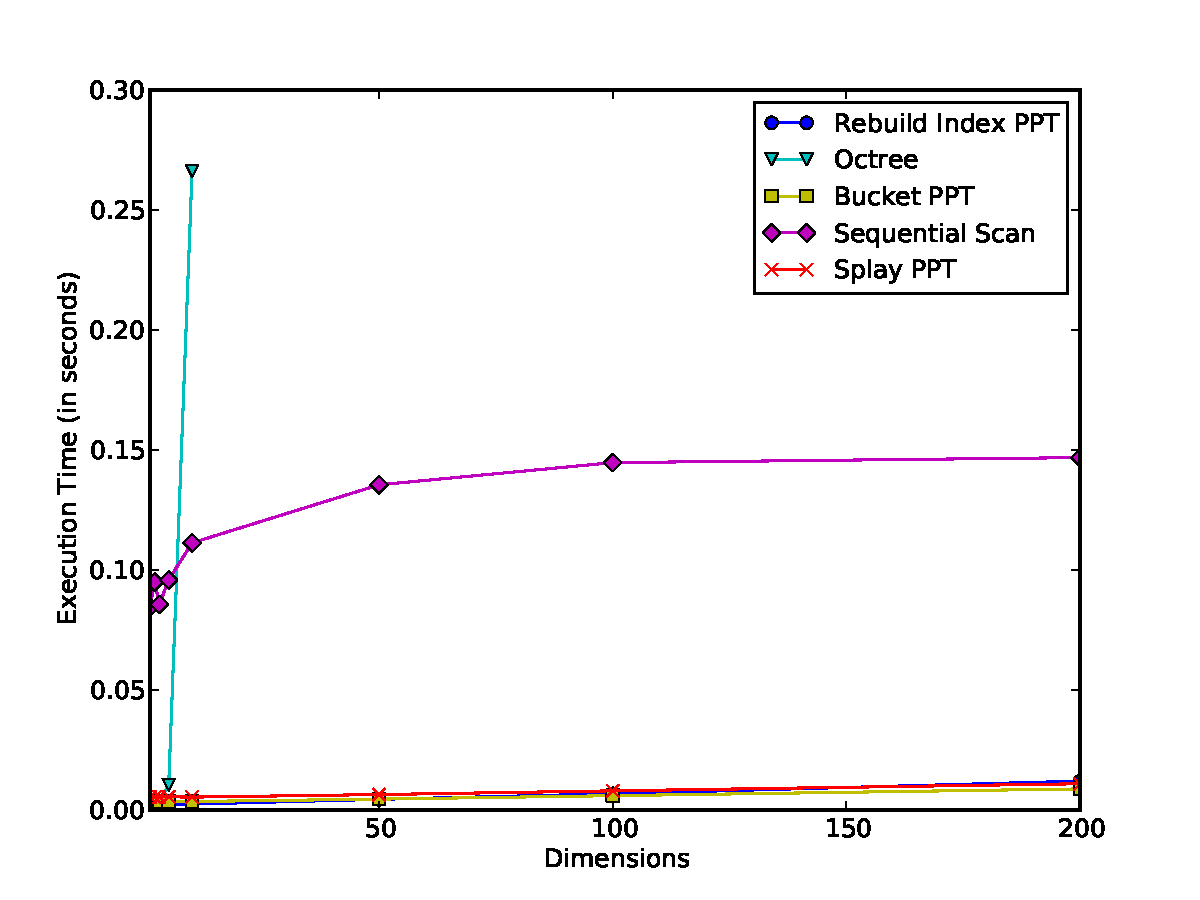
\includegraphics[scale=0.5]{figures/performance_analysis/iteration_1/randuniform_insert.pdf}
		}
		\end{subfloat}
		\begin{subfloat}[\texttt{delete}\label{fig:perf1-dimensionality-remove}]{%
			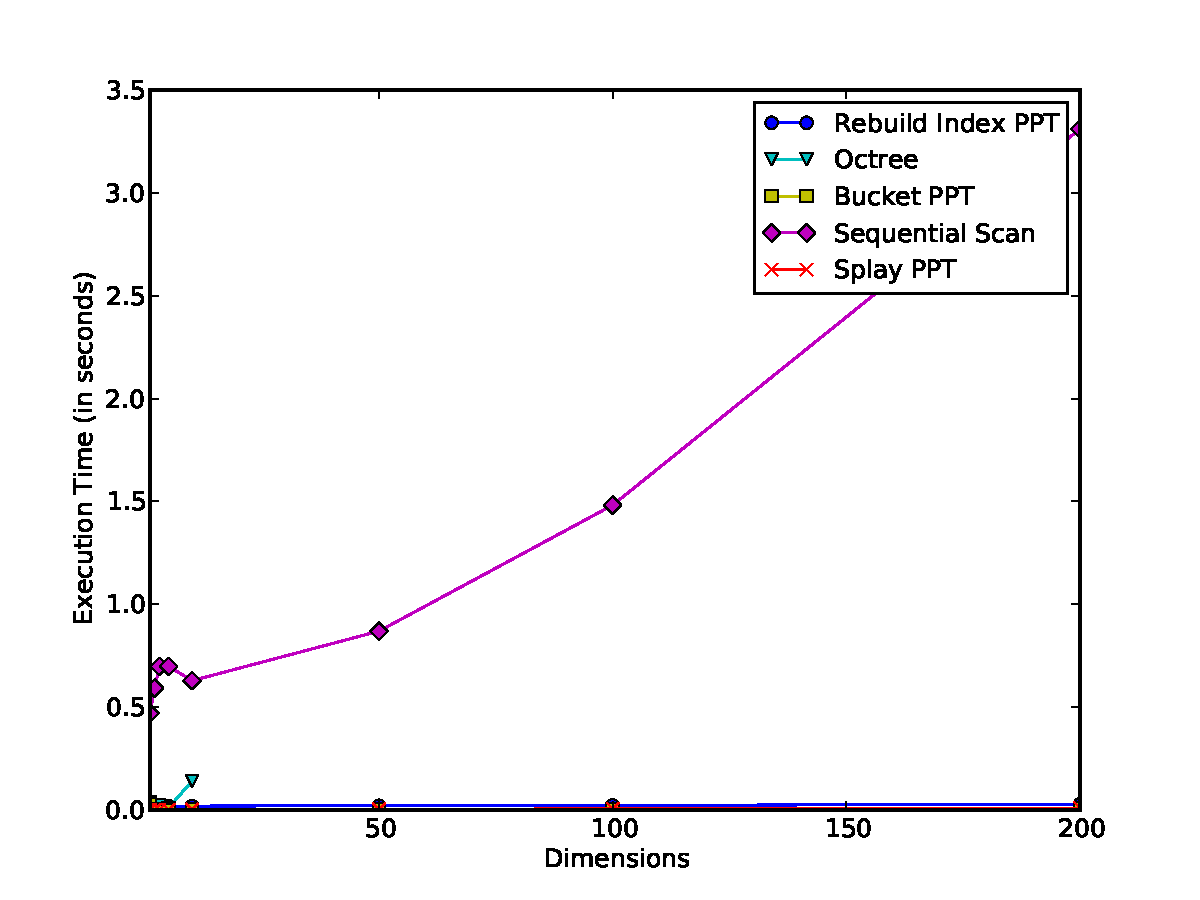
\includegraphics[scale=0.5]{figures/performance_analysis/iteration_1/randuniform_delete.pdf}
		}
		\end{subfloat}
	}%

	\caption{Index Structure Performance With Respect To Dimensionality (10,000 Points from Uniform Distribution Synthetic Dataset)}
	\label{fig:perf1-dimensionality}
\end{figure}

The two plots show that dimensionality has little effect on the performance of Sequential Scan. The speed of Sequential Scan decreases as $d$ is increased, which is because more computation needed for point comparisons, allocation and deallocation due an increased amount of data.

As expected, the Octree takes exponentially longer as $d$ increases, due to the exponential increase in nodes at each level ($2^d$ children per node). When $d > 10$, the number of excessive nodes was so high that the performance tests crashed because there was enough memory to store the exponentially increasing nodes.

All Pseudo-Pyramid Tree implementations have similar speeds for \texttt{insert} and point queries, which significantly outperform Sequential Scan and Octree. Like the baselines, the speed decreases as $d$ increases, but at a much slower rate than the Octree. Rebuild Index Pseudo-Pyramid Tree provides the slowest \texttt{delete}, due the tree having to be rebuilt after $R$ points are removed. The Bucket or Splay Pseudo-Pyramid Tree have the fastest deletion speed because they only require a single array deletion when deleting a point (each array stores much less than $n$ points if the hashing function discriminates well).

\begin{figure}
	\makebox[\textwidth][c]{%
		\begin{subfloat}[\texttt{insert}\label{fig:perf1-size-insert}]{%
			\begin{overpic}[scale=0.5]{figures/performance_analysis/iteration_1/sizevary_insert.pdf}
				\put(13,33){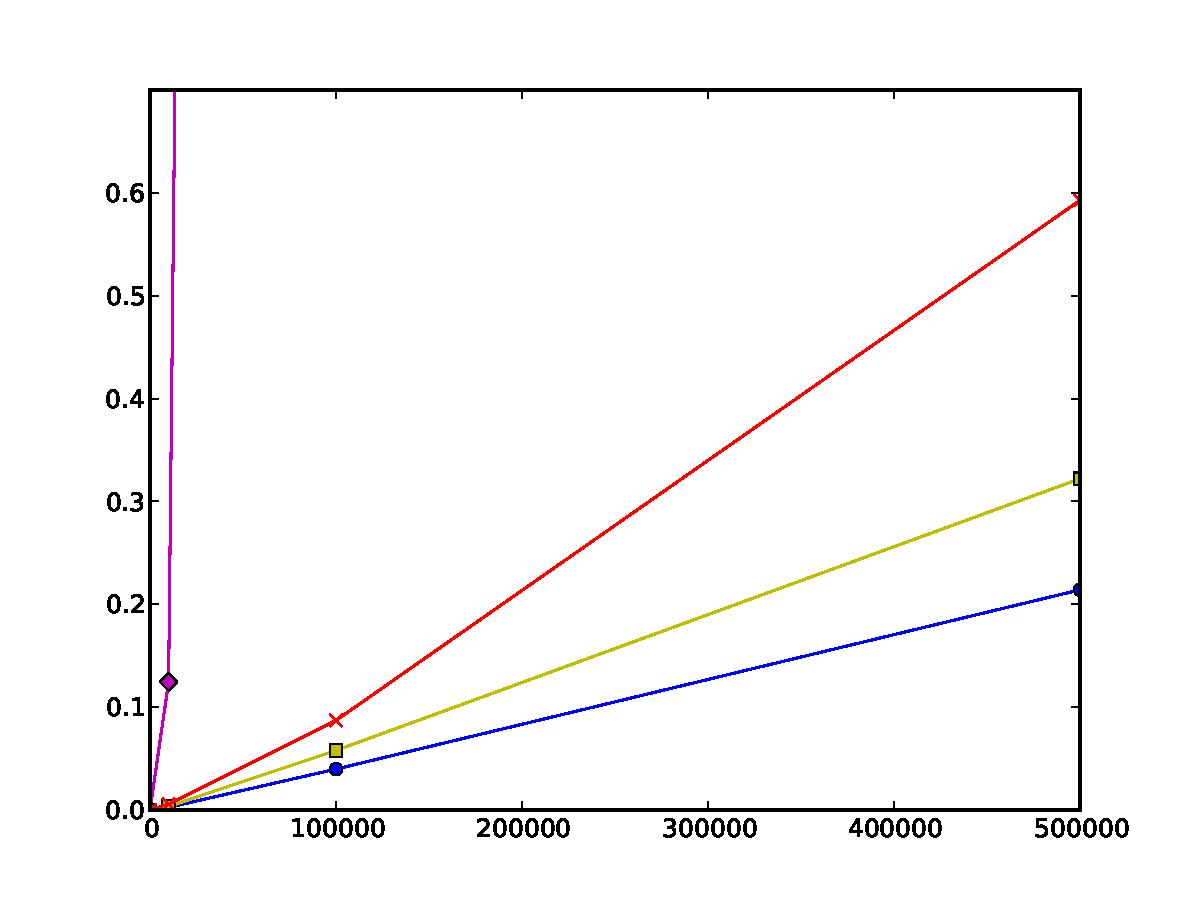
\includegraphics[scale=0.22]{figures/performance_analysis/iteration_1/sizevary_insert_zoomed.pdf}}
				\put(24,31){\textbf{\sans{Zoomed View}}}
			\end{overpic}
		}
		\end{subfloat}
		\begin{subfloat}[\texttt{delete}\label{fig:perf1-size-remove}]{%
			\begin{overpic}[scale=0.5]{figures/performance_analysis/iteration_1/sizevary_delete.pdf}
				\put(13,35){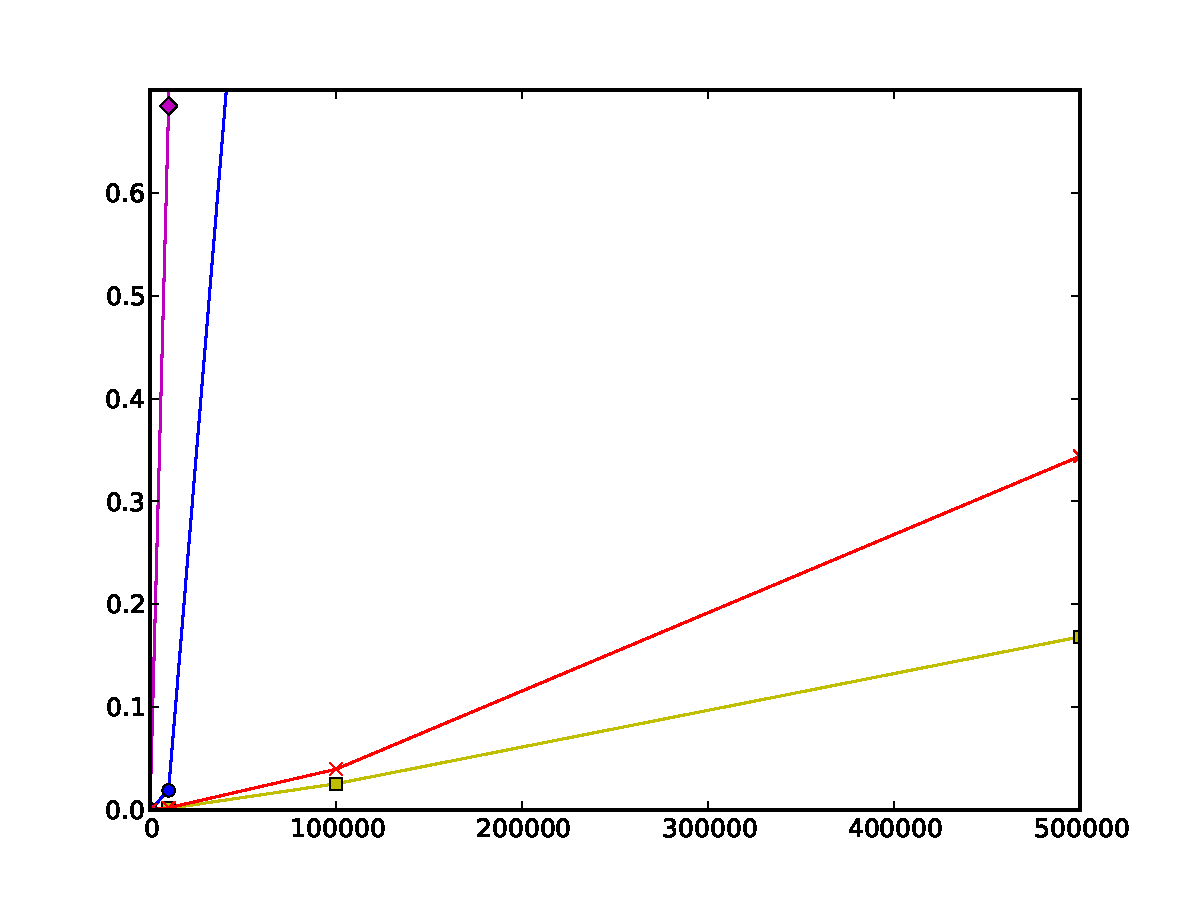
\includegraphics[scale=0.21]{figures/performance_analysis/iteration_1/sizevary_delete_zoomed.pdf}}
				\put(23,33){\textbf{\sans{Zoomed View}}}
			\end{overpic}
		}

		\end{subfloat}
	}%

	\caption{Index Structure Performance With Respect To Dataset Size (10,000 Points from Uniform Distribution Synthetic Dataset)}
	\label{fig:perf1-size}
\end{figure}

Execution times for the 16 dimension dataset of varying size is shown in Figure \ref{fig:perf1-size} (see Table \ref{tab:perf1-size} for exact execution times). Figure \ref{fig:perf1-size} shows that the speed of Sequential Scan decreases linearly with $n$. This is to be expected, as the complexity of its operations being $O(n)$.

The execution times for both operations with the Pseudo-Pyramid Tree variants grow very slowly as $n$ increases. This is likely because an operation's average complexity is $O(d)$ and dataset size only affects the performance of these operations if the tree's buckets become crowded with many points (as the buckets have to be searched to find the point). As $n$ is increased, \texttt{delete} speed decreases much faster in the Rebuild Pseudo-Pyramid Tree compared to the other Pseudo-Pyramid Tree implementations, since the time to rebuild the tree increases with $n$.

These results show storing separate point arrays for each bucket, instead of using one large array to store all the points, increases performance. Both the Bucket and Splay Pseudo-Pyramid Tree implementations provide faster \texttt{insert} and point query operations than the index-based rebuild implementation. As expected, this is due to an increased cache hit rate. Table \ref{tab:perf1-cache-hit-rate} displays the cache miss rate when \textit{inserting} 10,000 points into each Pseudo-Pyramid Tree implementation. Notice how the Rebuild Pseudo-Pyramid Tree, which stores indices in each bucket, has a greater cache miss rate. 

\begin{table}
	\centering
	\begin{tabular}{|l|l|}
		\hline
		\textbf{Structure} & \textbf{Cache Miss Rate (\%) (2 dp)} \\
		\hline
		Rebuild Pseudo-Pyramid Tree & 4.65 \\
		Bucket Pseudo-Pyramid Tree & 0.24 \\
		Splay Pseudo-Pyramid Tree & 0.59 \\
		\hline
	\end{tabular}
	\caption{Cache Hit Rate for \texttt{insert} Operations with Pseudo-Pyramid Variants (200D Randomly Uniform Dataset, 10,000 operations each)}
	\label{tab:perf1-cache-hit-rate}
\end{table}

The differences in speed between the bucket and splay tree implementations is small, but the Bucket Pseudo-Pyramid Tree slightly outperforms the Splay Tree with most datasets. Again, this may be due to having a lower cache miss rate. 

\subsection{Real Datasets and Impact of Bucket Size}

\begin{table}
	\centering
	\makebox[\textwidth][c]{%
		\begin{tabular}{|r|r|l|l|l|}
			\hline
			\multicolumn{2}{|c}{} & \multicolumn{3}{|c|}{\textbf{Dataset}} \\
			\hline
			\textbf{Structure} & \textbf{Operation} & \textbf{Astrophysics} & \textbf{Hurricane Isabel} & \textbf{Armadillo Mesh} \\
			\hline
			\multirow{4}{*}{Sequential Scan} & Delete & 1315.81 & 1920.73 & 1336.2 \\
				& Insert & 436.385 & 691.833 & 215.865 \\
				& Point Query & 435.88 & 651.428 & 212.585 \\
			\hline
			\multirow{4}{*}{Rebuild Index PPT} & Delete & 1856.11 & 2121.9 & 36.0037 \\
				& Insert & 139.346 & 117.441 & 0.112088 \\
				& Point Query & 139.048 & 117.292 & 0.0492687 \\
			\hline
			\multirow{4}{*}{Bucket PPT} & Delete & 82.908 & 14.9052 & 0.160532 \\
				& Insert & 81.231 & 14.4715 & 0.126938 \\
				& Point Query & 70.4391 & 14.3358 & 0.0956872 \\
			\hline
			\multirow{4}{*}{Splay PPT} & Delete & 88.4574 & 15.3893 & 0.203571 \\
				& Insert & 84.0908 & 14.7177 & 0.192196 \\
				& Point Query & 70.3729 & 14.6499 & 0.141219 \\
			\hline
		\end{tabular}
	}%

	\caption{Total Execution Time (in seconds) of Each Operation on Real Datasets}
	\label{tab:perf1-real}
\end{table}

Table \ref{tab:perf1-real} shows the runtime of each operation on sampled real datasets. Work gone into increasing the speed of the Pseudo-Pyramid Tree by exploring different implementations, which has worked to greatly accelerate the structure for most of the evaluation datasets. However, Table \ref{tab:perf1-real} shows that on the two scientific datasets, the relative speedup from Sequential Scan achieved by the Bucket Pseudo-Pyramid Tree appears low.

For example, $500,000$ point queries with the astrophysics dataset takes 435.88 seconds with Sequential Scan and 70.4391 seconds with the Bucket Pseudo-Pyramid Tree, meaning a speedup of $\frac{435.88}{70.4391} \approx 6.18$ has been achieved. Speedup for the hurricane Isabel dataset is slightly higher, being approximately 45.44. Compare these figures to the speedup gained with the armadillo mesh, which is 2221. With such a high speedup on some datasets, and the fact there exist algorithms which can perform search in $O(log_2 n)$ time, this raised an important question: why the speedup is so low?

Despite hashing a point taking $O(d)$ time, point queries will take much longer if there are large numbers of points in buckets. If each bucket contains exactly one point, then the complexity approaches $O(d)$. On the other extreme, where a single bucket contains all points, the complexity becomes $O(n)$. The number of points in a bucket, or \textit{bucket size}, is one of the most important factors to consider when analysing the performance of hash-based index structures. A ``good" hashing function tries to achieve an amortised running time of $O(1)$ by ensuring only one or two points are mapped to the same hash value.

\begin{table}
	\centering
	\begin{tabular}{|l|l|l|l|l|}
		\hline
		& & \multicolumn{3}{c|}{\textbf{Bucket Size Statistics}} \\
		\hline
		\textbf{Dataset} & \textbf{Time to Query (sec)} & \textbf{Average} & \textbf{Max} & \textbf{\#Buckets} \\
		\hline
		500,000 16D Random Points & 0.105091 & 1.0312 & 4 & 493488 \\
		500,000 Astrophysics Points & 70.4391 & 47820.89 & 153471 & 8  \\
		500,000 Hurricane Isabel Points & 14.3358 & 1257.46 & 154979 & 396 \\
		435,544 3D Armadillo Mesh Points & 0.141219 & 19.1465 & 187 & 22748 \\
		\hline
	\end{tabular}
	\caption{Statistics on Bucket Size with Pseudo-Pyramid Tree Based on Dataset}
	\label{tab:perf1-bucket-stats}
\end{table}

The mean, standard deviation, minimum and maximum bucket size has been used to determine if bucket size is the reason the Pseudo-Pyramid Tree is so slow for the astrophysics dataset. Table \ref{tab:perf1-bucket-stats} shows these statistics when the Pseudo-Pyramid Tree is storing points from one synthetic dataset and all the real datasets. There appears to be a relationship between average bucket size and the speed of the Pseudo-Pyramid Tree. The average bucket size for the scientific datasets go into the thousands for the scientific datasets, with the largest bucket containing 153471 and 497953 points using the astrophysics and hurricane datasets respectively. Notice how the time to query all points in the 16D random dataset takes the shorter time, due to the average bucket size being as small as 1.0312. These results match the observation that larger average bucket size means more computation must be performed per operation on average.

\subsection{Summary}

All Pseudo-Pyramid tree invariants greatly outperform the two baselines, with the Octree failing to store large numbers of points or points with more than 10 dimensions due to exponential memory requirements. The Rebuild Index Pseudo-Pyramid are clearly inferior to batch and splay, being slower for all three operations. While the Splay Pseudo-Pyramid Tree performs the fastest for some datasets, the Bucket Pseudo-Pyramid Tree performs the fastest on the majority of the datasets. Therefore, the Bucket Pseudo-Pyramid Tree will be used for any future evaluations.

With both scientific datasets, all Pseudo-Pyramid Tree variants degenerated to semi-sequential scan because they caused the hashing function to assign the same 1D value to a very large number of points. There appears to be a correlation between bucket size and the performance of hash-based structures. More research into decreasing bucket size by using different hashing functions should be performed to determine if hash-based structures can provide fast point queries for scientific datasets such as the astrophysics and hurricane Isabel simulations.